%%%%%%%%%%%%%%%%%%%%%%%%%%%%%%%%%%%%%%%%%
% Wenneker Article
% LaTeX Template
% Version 2.0 (28/2/17)
%
% This template was downloaded from:
% http://www.LaTeXTemplates.com
%
% Authors:
% Vel (vel@LaTeXTemplates.com)
% Frits Wenneker
%
% License:
% CC BY-NC-SA 3.0 (http://creativecommons.org/licenses/by-nc-sa/3.0/)
%
%%%%%%%%%%%%%%%%%%%%%%%%%%%%%%%%%%%%%%%%%

%----------------------------------------------------------------------------------------
%	PACKAGES AND OTHER DOCUMENT CONFIGURATIONS
%----------------------------------------------------------------------------------------

\documentclass[10pt, a4paper, twocolumn]{article} % 10pt font size (11 and 12 also possible), A4 paper (letterpaper for US letter) and two column layout (remove for one column)

%%%%%%%%%%%%%%%%%%%%%%%%%%%%%%%%%%%%%%%%%
% Wenneker Article
% Structure Specification File
% Version 1.0 (28/2/17)
%
% This file originates from:
% http://www.LaTeXTemplates.com
%
% Authors:
% Frits Wenneker
% Vel (vel@LaTeXTemplates.com)
%
% License:
% CC BY-NC-SA 3.0 (http://creativecommons.org/licenses/by-nc-sa/3.0/)
%
%%%%%%%%%%%%%%%%%%%%%%%%%%%%%%%%%%%%%%%%%

%----------------------------------------------------------------------------------------
%	PACKAGES AND OTHER DOCUMENT CONFIGURATIONS
%----------------------------------------------------------------------------------------

\usepackage{microtype} % Better typography

\usepackage{amsmath,amsfonts,amsthm} % Math packages for equations

\usepackage[svgnames]{xcolor} % Enabling colors by their 'svgnames'

\usepackage[hang, small, labelfont=bf, up, textfont=it]{caption} % Custom captions under/above tables and figures

\usepackage{booktabs} % Horizontal rules in tables

\usepackage{lastpage} % Used to determine the number of pages in the document (for "Page X of Total")

\usepackage{graphicx} % Required for adding images

\usepackage{enumitem} % Required for customising lists
\setlist{noitemsep} % Remove spacing between bullet/numbered list elements

\usepackage{sectsty} % Enables custom section titles

\usepackage{float}


\allsectionsfont{\usefont{OT1}{phv}{b}{n}} % Change the font of all section commands (Helvetica)

%----------------------------------------------------------------------------------------
%	MARGINS AND SPACING
%----------------------------------------------------------------------------------------

\usepackage{geometry} % Required for adjusting page dimensions

\geometry{
	top=1cm, % Top margin
	bottom=1.5cm, % Bottom margin
	left=2cm, % Left margin
	right=2cm, % Right margin
	includehead, % Include space for a header
	includefoot, % Include space for a footer
	%showframe, % Uncomment to show how the type block is set on the page
}

\setlength{\columnsep}{7mm} % Column separation width

%----------------------------------------------------------------------------------------
%	FONTS
%----------------------------------------------------------------------------------------

\usepackage[T1]{fontenc} % Output font encoding for international characters
\usepackage[utf8]{inputenc} % Required for inputting international characters

\usepackage{XCharter} % Use the XCharter font

%----------------------------------------------------------------------------------------
%	HEADERS AND FOOTERS
%----------------------------------------------------------------------------------------

\usepackage{fancyhdr} % Needed to define custom headers/footers
\pagestyle{fancy} % Enables the custom headers/footers

\renewcommand{\headrulewidth}{0.0pt} % No header rule
\renewcommand{\footrulewidth}{0.4pt} % Thin footer rule

\renewcommand{\sectionmark}[1]{\markboth{#1}{}} % Removes the section number from the header when \leftmark is used

%\nouppercase\leftmark % Add this to one of the lines below if you want a section title in the header/footer

% Headers
\lhead{} % Left header
\chead{\textit{\thetitle}} % Center header - currently printing the article title
\rhead{} % Right header

% Footers
\lfoot{} % Left footer
\cfoot{} % Center footer
\rfoot{\footnotesize Page \thepage\ of \pageref{LastPage}} % Right footer, "Page 1 of 2"

\fancypagestyle{firstpage}{ % Page style for the first page with the title
	\fancyhf{}
	\renewcommand{\footrulewidth}{0pt} % Suppress footer rule
}

%----------------------------------------------------------------------------------------
%	TITLE SECTION
%----------------------------------------------------------------------------------------

\newcommand{\authorstyle}[1]{{\large\usefont{OT1}{phv}{b}{n}\color{DarkRed}#1}} % Authors style (Helvetica)

\newcommand{\institution}[1]{{\footnotesize\usefont{OT1}{phv}{m}{sl}\color{Black}#1}} % Institutions style (Helvetica)

\usepackage{titling} % Allows custom title configuration

\newcommand{\HorRule}{\color{DarkGoldenrod}\rule{\linewidth}{1pt}} % Defines the gold horizontal rule around the title

\pretitle{
	\vspace{-30pt} % Move the entire title section up
	\HorRule\vspace{10pt} % Horizontal rule before the title
	\fontsize{32}{36}\usefont{OT1}{phv}{b}{n}\selectfont % Helvetica
	\color{DarkRed} % Text colour for the title and author(s)
}

\posttitle{\par\vskip 15pt} % Whitespace under the title

\preauthor{} % Anything that will appear before \author is printed

\postauthor{ % Anything that will appear after \author is printed
	\vspace{10pt} % Space before the rule
	\par\HorRule % Horizontal rule after the title
	\vspace{20pt} % Space after the title section
}

%----------------------------------------------------------------------------------------
%	ABSTRACT
%----------------------------------------------------------------------------------------

\usepackage{lettrine} % Package to accentuate the first letter of the text (lettrine)
\usepackage{fix-cm}	% Fixes the height of the lettrine

\newcommand{\initial}[1]{ % Defines the command and style for the lettrine
	\lettrine[lines=3,findent=4pt,nindent=0pt]{% Lettrine takes up 3 lines, the text to the right of it is indented 4pt and further indenting of lines 2+ is stopped
		\color{DarkGoldenrod}% Lettrine colour
		{#1}% The letter
	}{}%
}

\usepackage{xstring} % Required for string manipulation

\newcommand{\lettrineabstract}[1]{
	\StrLeft{#1}{1}[\firstletter] % Capture the first letter of the abstract for the lettrine
	\initial{\firstletter}\textbf{\StrGobbleLeft{#1}{1}} % Print the abstract with the first letter as a lettrine and the rest in bold
}

%----------------------------------------------------------------------------------------
%	BIBLIOGRAPHY
%----------------------------------------------------------------------------------------
\usepackage[backend=bibtex,natbib=true]{biblatex} % Use the bibtex backend with the authoryear citation style (which resembles APA)

\addbibresource{Reference.bib} % The filename of the bibliography

\usepackage[autostyle=true]{csquotes} % Required to generate language-dependent quotes in the bibliography
 % Specifies the document structure and loads requires packages

%----------------------------------------------------------------------------------------
%	ARTICLE INFORMATION
%----------------------------------------------------------------------------------------

\title{Improved Method for Binaural Rendering Based on Parametric Processing} % The article title

\author{
	\authorstyle{Chuhan Qiu\textsuperscript{1}} % Authors
	\newline\newline % Space before institutions
	\textsuperscript{1}\institution{Communication University of China, Beijing, China}\\ % Institution 1
}

% Example of a one line author/institution relationship
%\author{\newauthor{John Marston} \newinstitution{Universidad Nacional Autónoma de México, Mexico City, Mexico}}

\date{} % Add a date here if you would like one to appear underneath the title block, use \today for the current date, leave empty for no date

%----------------------------------------------------------------------------------------

\begin{document}

\maketitle % Print the title

\thispagestyle{firstpage} % Apply the page style for the first page (no headers and footers)

%----------------------------------------------------------------------------------------
%	ABSTRACT
%----------------------------------------------------------------------------------------

\lettrineabstract{Parametric processing is a kind of method based on sound field modelling and perceptually motivated, which has wide applicability in spatial audio. Commonly, parametric processing utilizes adaptive filter to extract specific parameters and signals from the assumed sound field model, which is typically represented by the signals captured by microphone array. In this paper, we propose a rendering method based on parametric information processing and optimized HRTF filter, which enhances the articulation and spatial perception effect.}

%----------------------------------------------------------------------------------------
%	ARTICLE CONTENTS
%----------------------------------------------------------------------------------------

\section{INTRODUCTION}

In sound recording, we commonly use multiple microphones to reproduce the sound sources and their position in real sound field. The coverage angle, placement position, pointing angle and quantity of the microphones determine the different microphone techniques. Correspondingly, the captured signals' processing methods and the effect of them are completely different as well. Spatial audio recordings have specific microphone setups and focus on the reconstruction of the acoustic fields. In processing stage, as so called spatial audio rendering, we want to better reproduce the performance of the sound sources and acoustic field, mainly manifested as whether the position of the virtual sound source is accurate and the spatial perception is close to reality, etc. Based on these premises, many methods have been proposed to enhance the performance of spatial information, and parametric spatial processing is usually a flexible and efficient solution for most sound scene.

The stepping stone in development of parametric spatial audio techniques is based on decomposing the spatial impulse response rendering (SIRR) into one direct sound and a diffuse residual for each time-frequency bin~\parencite{Reference1}. The underlying theoretical basis of this method actually assumes that source signals tend to be sparse in the time-frequency domain, especially for signals with obvious harmonic structures, e.g. music and speech. 


%------------------------------------------------
%------------------------------------------------
\section{METHOD}

~\parencite{Reference2} proposed directional audio coding (DirAC), whose assumed sound field model is obtained from a zeroth-order (omnidirectional) signal and two parameters: the DOA (Direction-of-Arrival) and the diffuse. DirAC is a processing solution for B-format (1st-order Ambisonics), which totally has four channels.
\begin{align}
& W = S \cdot \frac{1}{\sqrt{2}} \\
& X = S \cdot cos{\theta}cos{\phi} \\
& Y = S \cdot sin{\theta}cos{\phi} \\
& Z = S \cdot sin{\phi}
\end{align}

\begin{figure*}
	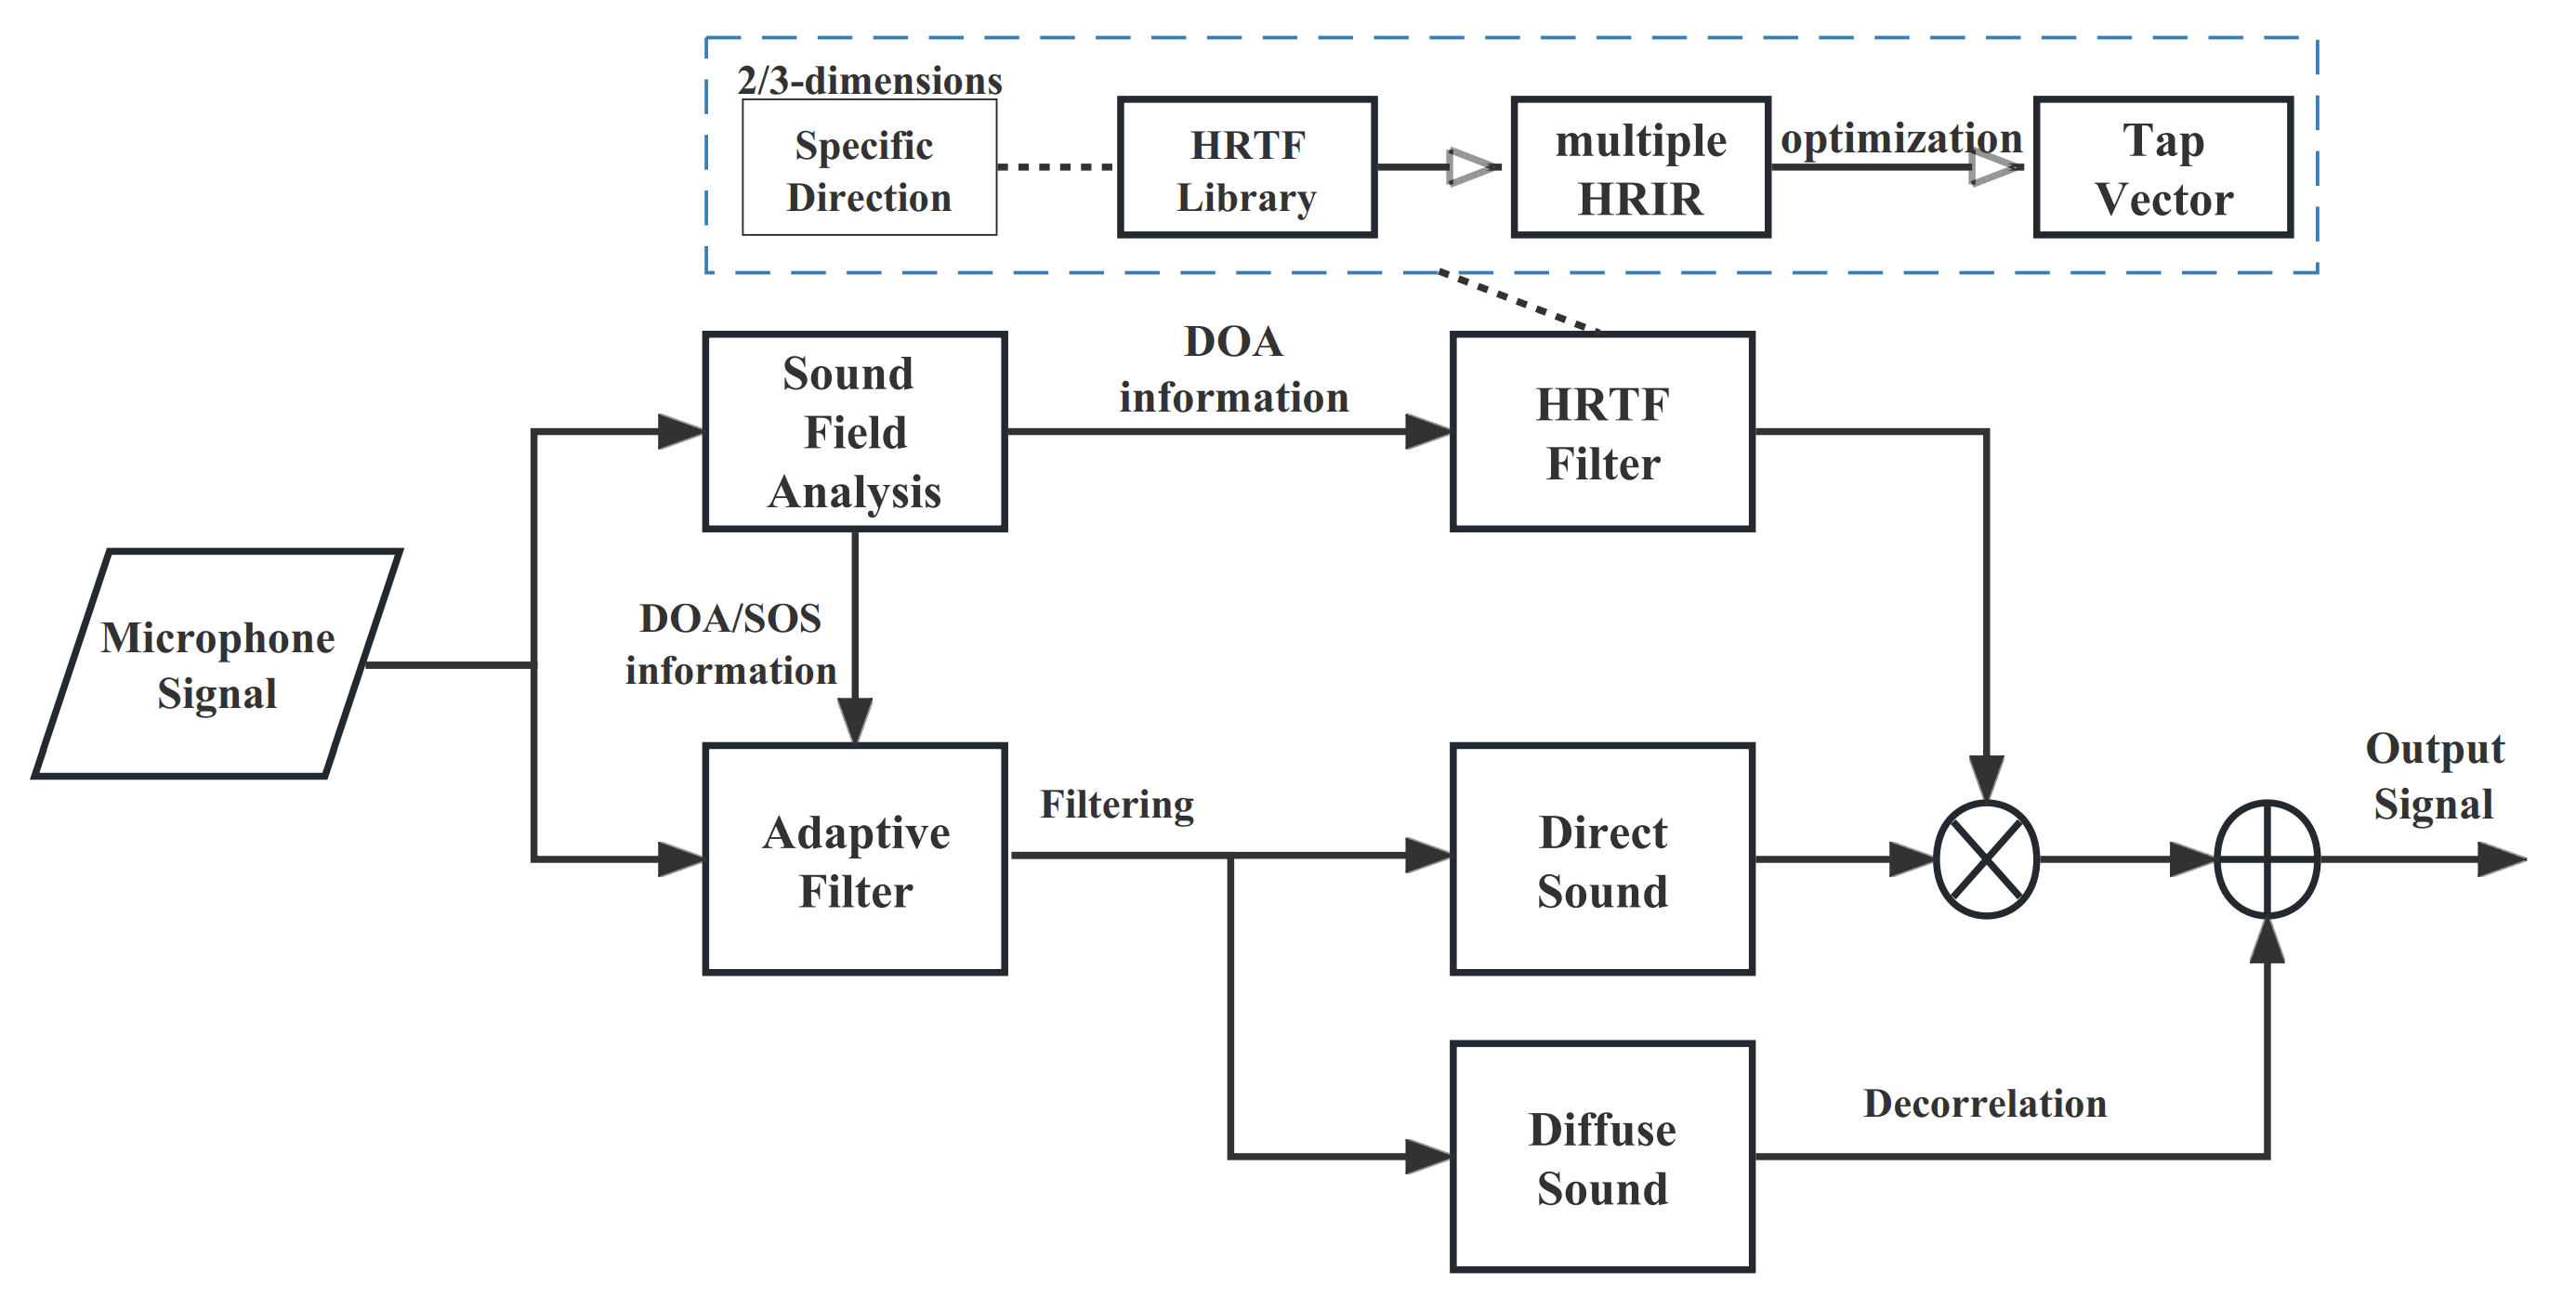
\includegraphics[width=\linewidth]{Figure1.png} % Figure image
	\caption{Flow chart of the improved method for binaural rendering} % Figure caption
	\label{bear} % Label for referencing with \ref{bear}
\end{figure*}

Obviously, $W$ signal corresponds to the omnidirectional microphone, whereas $XYZ$ are the components along three spatial axes. In this way, DirAC utilizes $XYZ$ to estimate the intensity vector $i$, and estimates the sound field energy density $e$ in conjunction with $W$. Then, the DOA and the diffuse $\varphi$ can be further derived from $i$ and $e$.
\begin{align}
DOA = -\angle{E[i]} \\
\varphi = 1 - \frac{||E[i]||}{cE[e]}
\end{align}
where the operator $\angle$ gives the 3D angle of a vector, and $E[\;]$ is the expectation operator.

DirAC is a classical example of parametric spatial audio, which obtain a perceptive meaningful description of the recording sound field by extracting the direct and diffuse sound components and some parametric information~\cite{Reference3}. We may use single-channel or multi-channel adaptive filter to extract the direct and diffuse signal components and other parametric information from the mono $W$ signal or other signals captured by different microphone arrays, then updating the tap weights of the adaptive filters which enable the filters to adapt to fast changing acoustics and provide a good trade-off between robustness and attenuation of undesired signals~\parencite{Reference4}. 

Figure 1 shows the whole flow chart of the method proposed in this paper, and each module of it is explained separately in the following sections.


%------------------------------------------------
\subsection{Adaptive Spatial Filter}

Both Single-channel filter and multi-channel filter can be used for the extraction of direct and diffuse sound signal. To compute the tap weights of the filters, we may exploit knowledge about the DOA estimate of the direct sound or the second-order-statistics (SOS) information of the sound field~\parencite{Reference3}. Commonly, in single-channel filter, the signal-to-diffuse ratio $SDR(k,n)$ or the diffuseness $\psi(k,n)$ need to be estimated. And in multi-channel filter, more parameters are required include the DOA $\theta(k,n)$ of the direct sound, the diffuse sound power $\phi_d(k,n)$ and the PSD matrix $\Phi_n(k)$ of slowly time-varying noise.

\subsubsection{Single-channel filter}

Based on single-channel filter, we can estimate the direct and the diffuse components effectively, which is actually by applying a spectral gain factor to a single microphone signal.The direct signal estimation can be expressed as 
\begin{equation}
\hat{X}_s(k, n, d_1) = W_s(k, n)X(k, n, d_1)
\end{equation}
where $W_s(k,n)$ is the single-channel filter, which is multiplied with the reference microphone signal to obtain the direct sound at $d_1$. 

We may obtain the optimal filter by minimizing the mean-square error between the true and estimated direct sound, which yields the well-known Wiener filter (WF). 

\subsubsection{Multi-channel filter}

Different from single-channel filter, multi-channel filter recomputes the tap weights each time and frequency with updated information on the DOA and second-order-statistics. Multi-filter can adapt fast to changing acoustics and overcome many limitations of the single-channel filter. The direct sound estimated by multi-channel filter is
\begin{equation}
\hat{X}_s(k,n,d_1) = w_s^H(k,n) x(k,n)
\end{equation}

To obtain the optimal filter $w_s$, there are two filter types: the linearly-constrained minimum variance (LCMV) filter and  the parametric multi-channel Wiener filter. For LCMV filter, the optimal filter can be found by minimizing the noise-plus-diffuse power while extracting the distortionless response for the direct sound
\begin{equation}
\begin{split}
&w_{sLCMV}(k,n) = arg_{w_s}min\,{w_s^H}[\Phi_d(k,n)+ \Phi_n(k)]w_s \\
&s.t.\; w_s^H(k,n)v(k,n) = 1
\end{split}
\end{equation}
where the propagation vector$v(k,n)$ depends on the array geometry and DOA $\theta(k,n)$ of the direct sound. 

For multi-channel Wiener filter, the loss function is the same as single-channel Wiener filter but with a linear constraint
\begin{equation}
\begin{split}
& w_{sPMW}(k,n) = arg_{w_s}min\,{w_s^H}[\Phi_d(k,n)+ \Phi_n(k)]w_s \\
& s.t.\;E\{|w_s^H(k,n)x_s(k,n) - P_s(k,n,d_1)|^2\} \leq \sigma^2(k,n)
\end{split}
\end{equation}

Here, both in (9) and (10), $\Phi_d(k,n)$ is the power spectral density (PSD) matrix of the diffuse sound, which can be written as
\begin{equation}
\begin{split}
\Phi_d(k,n) &= E\{x_d(k,n)x_d^H(k,n)\} \\
&= \phi_d(k,n) \Gamma_d(k)
\end{split}
\end{equation}
where $\phi_d(k,n)$ is the power of the diffuse sound and $\Gamma_d(k)$ is the diffuse sound coherence matrix. When assuming a specific diffuse field characteristic, each elements of $Gamma_d(k)$ is typically known a priori. In this way, to compute the loss function of the diffuse sound, we mainly need to obtain the power of the diffuse sound $\phi_d(k,n)$ and the PSD matrix of the noise $\Phi_n(k)$.


%------------------------------------------------
\subsection{Sound Field Analysis}

As what has been told in last section, the parameters need to be extracted in sound field analysis stage depend on the type of adaptive spatial filter we used

\begin{description}
    \item[Single-channel Wiener filter] signal-to-diffuse ratio $SDR(k,n)$ or the diffuseness $\psi(k,n)$
    \item[LCMV filter] DOA $\theta(k,n)$ of the direct sound, diffuse sound power $\phi_d(k,n)$ and PSD matrix $Phi_n(k)$
\end{description}

%------------------------------------------------
\subsection{HRTF Filter}

In the application of binaural rendering, blocking the input signal and convolution it with HRIR is a very common method. However, this still causes much performance overhead compared to directly use the tap weights for filtering. A simple test in Matlab has been shown in Figure 2, which reflects the time cost between filtering by convolution and by tap weights. Obviously, in most cases, the latter takes an order of magnitude less time that the former.

\begin{table}[htbp]
	\centering
	\caption{Running time cost of different filtering method (average value)}
	\begin{tabular}{cccc}
		\toprule  
		Filter Order & Convolution & Tap Weights \\ 
		\midrule  % 中部线
		2nd-order & 0.006276 & 0.000451 \\
		\midrule 
		5th-order & 0.006341 & 0.000761 \\
	    \midrule  
	    10th-order & 0.006375 & 0.000762 \\
	    \midrule 
	    15th-order & 0.007016 & 0.000861 \\
		\bottomrule  % 底部线
	\end{tabular}
\end{table}

As shown in Figure 1, we obtain the tap vectors of HRIR by optimization algorithm~\parencite{Reference5}. In rendering stage, we select the HRIR tap vector closest to the DOA direction estimated by sound field analysis module, and filtering the direct sound extracted by adaptive spatial filter.

The iteration of multi-direction HRIR is also a part of the time cost. So we may reduce the HRIR quantity by choosing more representative directions appropriately. And for 2-D reproduction rendering, we only select the horizontal plane HRIR. Only when 3-D playback is required and introduce the HRIR with evaluation. All selected direction HRIRs will be pre calculated and stored, and only need to be called during real-time rendering.

To prevent the problem may caused by phase distortion and feedback loops, the tap vectors of HRIRs only include numerator coefficients, i.e. using FIR filters.

%------------------------------------------------
\subsection{Direct Sound Synthesis}

After obtaining the corresponding direction HRIR tap weights, we synthesise the final direct sound by filtering the direct sound using HRTF filter estimated. As what has been proved in Matlab, this method could reduce much time for computing in real-time.

%------------------------------------------------
\subsection{Diffuse Sound Synthesis}

Binaural reproduction includes only two channels, but decorrelation still plays an very import role. Decorrelation is important  for auditory spatial impression~\parencite{Reference6}~\parencite{Reference7}, and can extend the size of the listening area in loudspeaker reproduction which is less important in binaural reproduction because the listener is always at the sweet point~\parencite{Reference7}.

The decorrelation can be implemented using frequency-dependent delays, and the result is a signal that has a random delay at each frequency band but the magnitude response has not been changed\parencite{Reference8}. To prevent the decorrelation contributing to the perception of direction or spaciousness, the delays are within eligible boundaries.


%------------------------------------------------
%------------------------------------------------
\section{IMPLEMENTATION}

At present, the collection of theories has been relatively comprehensive. At the same time, various factors have been considered and a large number of review documents have been used for reference. However, in the actual implementation process, several problems have emerged. Due to time constraints, a lot of time and energy have been spent in the literature research stage, so this assignment does not give a complete implementation process. The implementation ideas have been fully introduced in the previous article. The main implementation difficulties will be introduced in the appendix of this submission.



%----------------------------------------------------------------------------------------
%	BIBLIOGRAPHY
%----------------------------------------------------------------------------------------

\printbibliography% Print the bibliography, section title in curly brackets

%----------------------------------------------------------------------------------------

\end{document}
